\section{TextSeal 2: Direct top-10
resampling}\label{record-docs-watermarking-qualitative-text-textseal2-direct-topk-md-textseal-2-direct-top-10-resampling}

This is a fresh answer to the same prompt, not a rewrite.

Eight pairs selected by fixed test positions before inspecting detection
or quality outcomes. Undetected originals and unsuccessful attacks
remain included.

\begin{recordfigure}
\centering
\pandocbounded{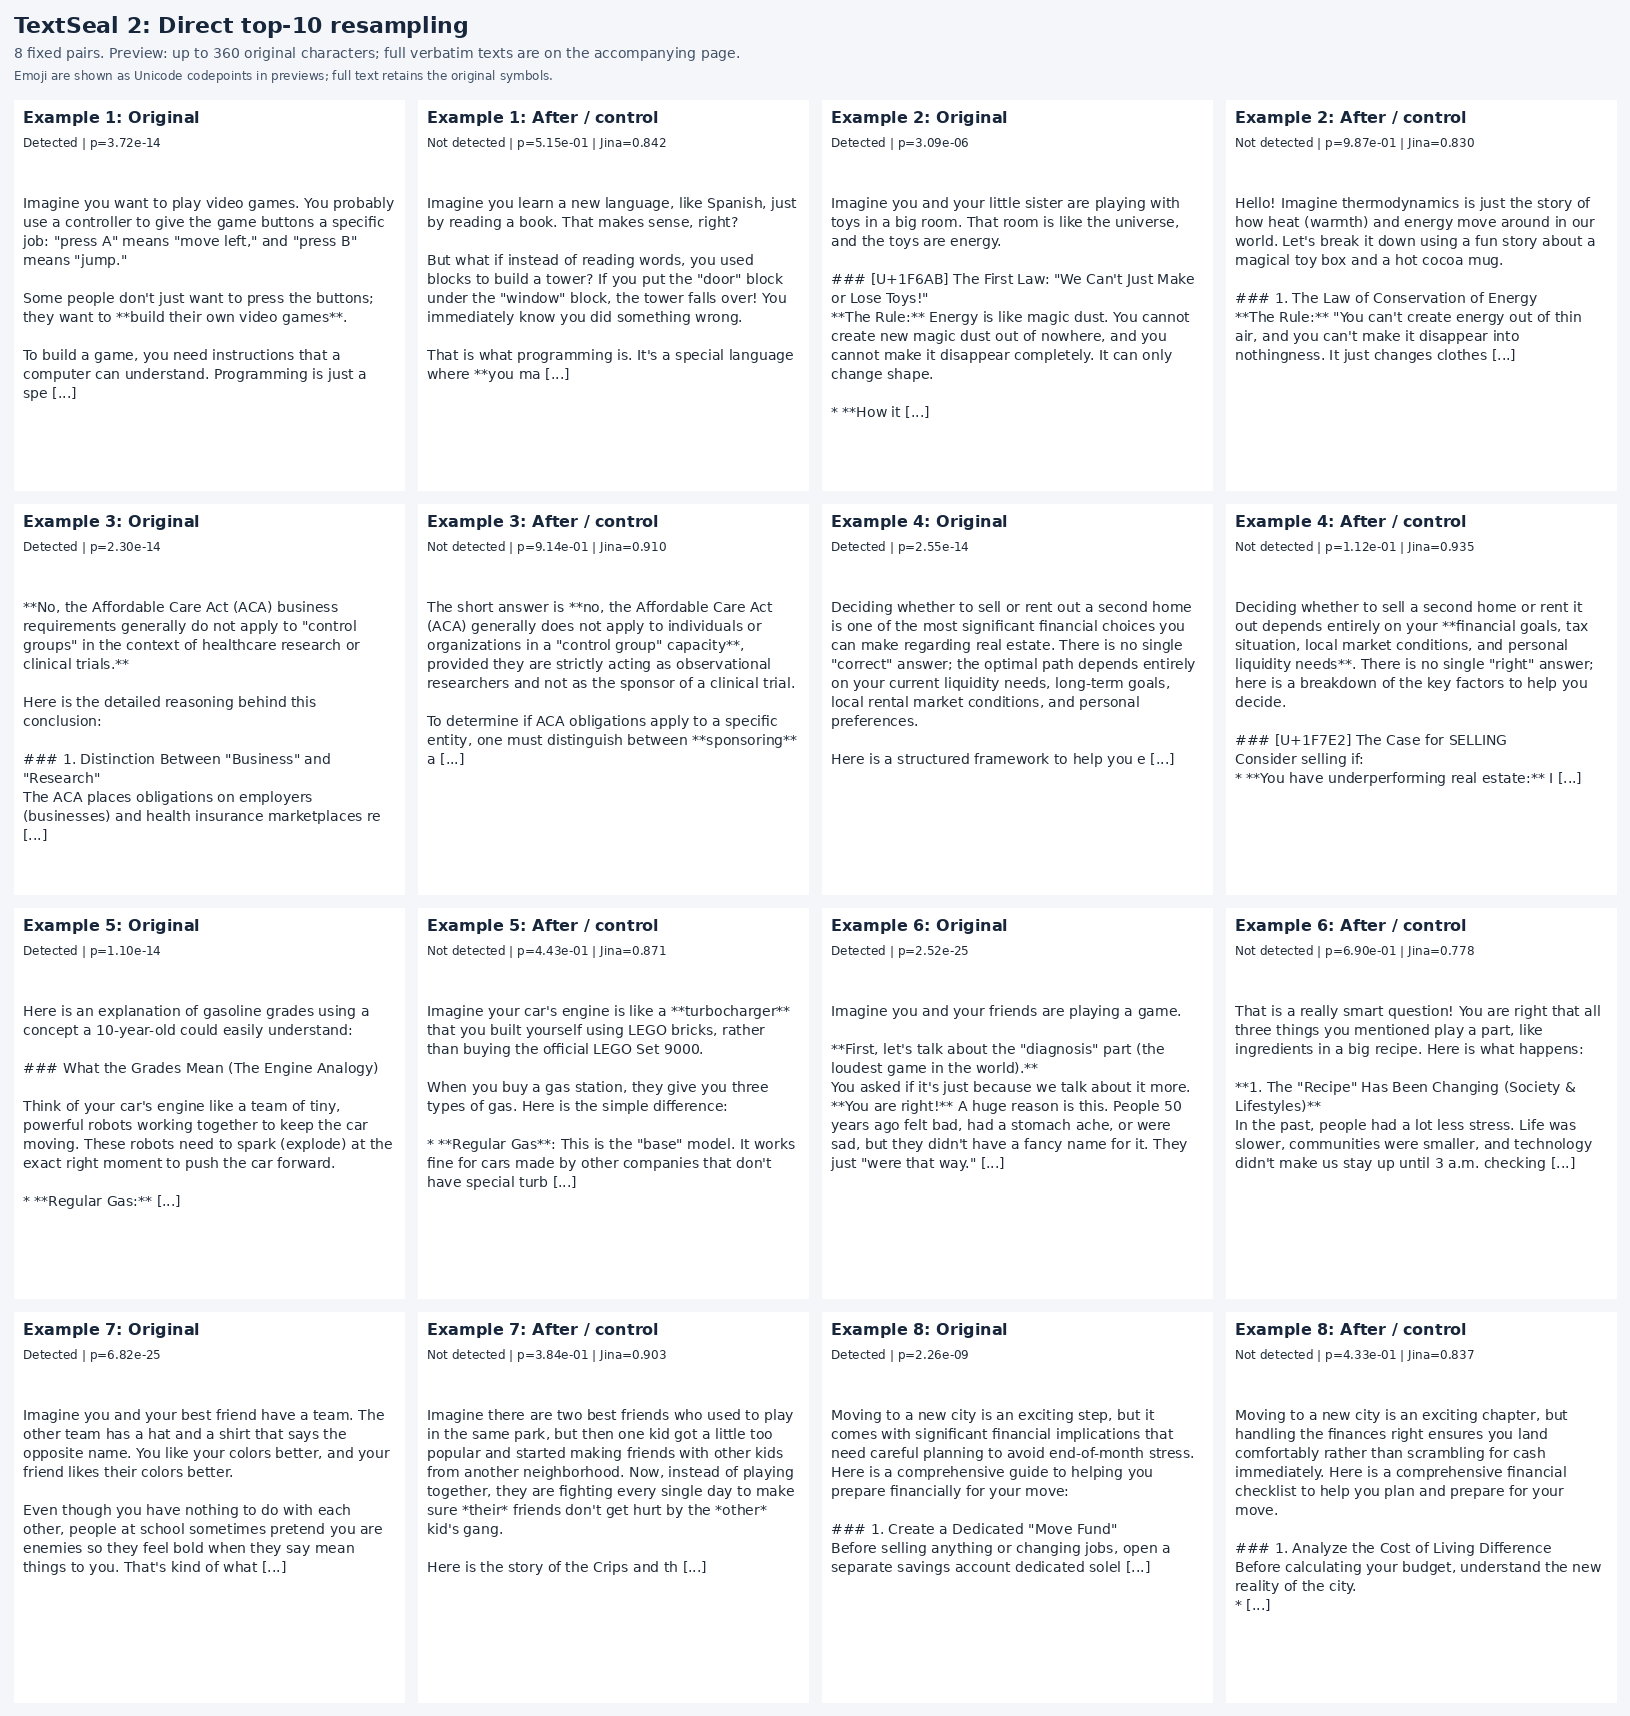
\includegraphics[keepaspectratio,alt={Sixteen-panel text preview}]{figures/text-textseal2-direct_topk.png}}
\caption{Sixteen-panel text preview}
\end{recordfigure}

The figure previews up to the first 360 original characters per
response; full texts below are unabridged. Emoji use Unicode codepoints
in the preview to avoid missing-glyph boxes. Owner scores and quality
metrics use full responses.

{\scriptsize\setlength{\tabcolsep}{3pt}\def\LTcaptype{none} % do not increment counter
\begin{longtable}[]{@{}
  >{\raggedright\arraybackslash}p{(\linewidth - 8\tabcolsep) * \real{0.2000}}
  >{\raggedright\arraybackslash}p{(\linewidth - 8\tabcolsep) * \real{0.2000}}
  >{\raggedright\arraybackslash}p{(\linewidth - 8\tabcolsep) * \real{0.2000}}
  >{\raggedright\arraybackslash}p{(\linewidth - 8\tabcolsep) * \real{0.2000}}
  >{\raggedright\arraybackslash}p{(\linewidth - 8\tabcolsep) * \real{0.2000}}@{}}
\toprule\noalign{}
\begin{minipage}[b]{\linewidth}\raggedright
Example
\end{minipage} & \begin{minipage}[b]{\linewidth}\raggedright
Test position
\end{minipage} & \begin{minipage}[b]{\linewidth}\raggedright
Before
\end{minipage} & \begin{minipage}[b]{\linewidth}\raggedright
After
\end{minipage} & \begin{minipage}[b]{\linewidth}\raggedright
Jina
\end{minipage} \\
\midrule\noalign{}
\endhead
\bottomrule\noalign{}
\endlastfoot
1 & 0 & Detected \textbar{} p=3.72e-14 & Not detected \textbar{}
p=5.15e-01 & 0.8415 \\
2 & 32 & Detected \textbar{} p=3.09e-06 & Not detected \textbar{}
p=9.87e-01 & 0.8304 \\
3 & 64 & Detected \textbar{} p=2.30e-14 & Not detected \textbar{}
p=9.14e-01 & 0.9096 \\
4 & 96 & Detected \textbar{} p=2.55e-14 & Not detected \textbar{}
p=1.12e-01 & 0.9350 \\
5 & 128 & Detected \textbar{} p=1.10e-14 & Not detected \textbar{}
p=4.43e-01 & 0.8714 \\
6 & 160 & Detected \textbar{} p=2.52e-25 & Not detected \textbar{}
p=6.90e-01 & 0.7778 \\
7 & 192 & Detected \textbar{} p=6.82e-25 & Not detected \textbar{}
p=3.84e-01 & 0.9034 \\
8 & 224 & Detected \textbar{} p=2.26e-09 & Not detected \textbar{}
p=4.33e-01 & 0.8371 \\
\end{longtable}
}

\subsection{Example 1: test position
0}\label{record-docs-watermarking-qualitative-text-textseal2-direct-topk-md-example-1-test-position-0}

Prompt ID:
\texttt{\seqsplit{eb41610306c3726e0a74a6888b55bc82ea505683f3fe908e286b197665852b84}}.

\textbf{Question / prompt}

\begin{Verbatim}
Why do people want programming taught in elementary / high schools ? I know absolutely nothing about programming . EDIT : I 'm marking this as answered . Thanks to everyone who replied ! Explain like I'm five.
\end{Verbatim}

\textbf{Original watermarked-model output}

\begin{Verbatim}
Imagine you want to play video games. You probably use a controller to give the game buttons a specific job: "press A" means "move left," and "press B" means "jump."

Some people don't just want to press the buttons; they want to **build their own video games**.

To build a game, you need instructions that a computer can understand. Programming is just a special language that tells the computer what to do. It's like writing the "rulebook" for the computer to follow.

People teach this to kids because:
1.  **It's a superpower:** Just like learning to speak English helps you talk to friends, learning code helps you talk to computers.
2.  **It builds good habits:** Programming teaches kids to be very patient (computers don't have feelings!) and to solve puzzles step-by-step, just like solving a math problem.
3.  **It changes how the world works:** Soon, they
\end{Verbatim}

\textbf{After / alternative output}

\begin{Verbatim}
Imagine you learn a new language, like Spanish, just by reading a book. That makes sense, right?

But what if instead of reading words, you used blocks to build a tower? If you put the "door" block under the "window" block, the tower falls over! You immediately know you did something wrong.

That is what programming is. It's a special language where **you make mistakes, and the computer tells you exactly what to fix.**

People want to teach this in school for three big reasons:

1.  **It's a Super Skill for the Future**
    Think about a job where you are an artist, a musician, or even just someone who loves reading books in the future. Being able to use your brain to solve puzzles and follow logical steps (like a computer needs) will help you succeed in *any* job, not just jobs that require typing code all day.

2.  **It Teaches You How to Think
\end{Verbatim}

Recorded diagnostics:
\texttt{\seqsplit{\{"mistral\_perplexity": 8.125\}}}.

\subsection{Example 2: test position
32}\label{record-docs-watermarking-qualitative-text-textseal2-direct-topk-md-example-2-test-position-32}

Prompt ID:
\texttt{\seqsplit{55ce85cdcf38f9b189c667d07ffb34cc5bd73600e98a2987c721e3a8c166c343}}.

\textbf{Question / prompt}

\begin{Verbatim}
Thermodynamics Could someone explain to me the first , and second laws of thermodynamics , and conservation of energy ? Explain like I'm five.
\end{Verbatim}

\textbf{Original watermarked-model output}

\begin{Verbatim}
Imagine you and your little sister are playing with toys in a big room. That room is like the universe, and the toys are energy.

### [U+1F6AB] The First Law: "We Can't Just Make or Lose Toys!"
**The Rule:** Energy is like magic dust. You cannot create new magic dust out of nowhere, and you cannot make it disappear completely. It can only change shape.

*   **How it works:** If you blow up a balloon, you used energy from your breath to make the rubber stretch. If that balloon pops, the energy doesn't vanish; it turns into a tiny *whoosh* of sound and a little bit of heat warming up the room.
*   **The Secret:** The total amount of toys in the whole room stays exactly the same forever. Energy just changes clothes (from movement to heat, from heat to light), but the total number never goes up or down.

### [U+1F504] The Second Law: "The Toys
\end{Verbatim}

\textbf{After / alternative output}

\begin{Verbatim}
Hello! Imagine thermodynamics is just the story of how heat (warmth) and energy move around in our world. Let's break it down using a fun story about a magical toy box and a hot cocoa mug.

### 1. The Law of Conservation of Energy
**The Rule:** "You can't create energy out of thin air, and you can't make it disappear into nothingness. It just changes clothes."

Imagine you have **$100** in your pocket.
*   If you buy an ice cream for $10, you now have $90 and an ice cream. Where did the ice cream come from? It came from the $10 you spent!
*   The money didn't disappear; it just turned into ice cream flavor.
*   The same is true for energy. If you eat an apple, the chemical energy in the apple doesn't vanish. It turns into your movement, your heat, and maybe even a
\end{Verbatim}

Recorded diagnostics:
\texttt{\seqsplit{\{"mistral\_perplexity": 6.21875\}}}.

\subsection{Example 3: test position
64}\label{record-docs-watermarking-qualitative-text-textseal2-direct-topk-md-example-3-test-position-64}

Prompt ID:
\texttt{\seqsplit{3cd335e45281f1d50700d93f931fc20b2f8fef24b7084ab3b583f745105137b1}}.

\textbf{Question / prompt}

\begin{Verbatim}
Do Affordable Care Act business requirements apply to “control groups?”
\end{Verbatim}

\textbf{Original watermarked-model output}

\begin{Verbatim}
**No, the Affordable Care Act (ACA) business requirements generally do not apply to "control groups" in the context of healthcare research or clinical trials.**

Here is the detailed reasoning behind this conclusion:

### 1. Distinction Between "Business" and "Research"
The ACA places obligations on employers (businesses) and health insurance marketplaces regarding health coverage mandates, minimum essential coverage (MEC), and marketplaces. These are statutory requirements designed to regulate the market and prevent bare minimum coverage scenarios.

"Control groups," however, are a fundamental concept in **clinical research, epidemiology, and data science**. They are cohorts of individuals used in scientific studies to compare the effects of an intervention (treatment) against a baseline to establish causality. They are not inherently "business entities" (like an employer or insurance carrier) subject to ACA compliance rules regarding hiring, insurance purchasing, or marketplace enrollment.

### 2. Specific Contexts Where ACA Might Interfere
\end{Verbatim}

\textbf{After / alternative output}

\begin{Verbatim}
The short answer is **no, the Affordable Care Act (ACA) generally does not apply to individuals or organizations in a "control group" capacity**, provided they are strictly acting as observational researchers and not as the sponsor of a clinical trial.

To determine if ACA obligations apply to a specific entity, one must distinguish between **sponsoring** a research study and **participating** as a control group within it. Here is the breakdown of how the ACA interacts with control groups:

### 1. The Distinction: Sponsor vs. Participant
Under federal law (42 CFR § 446.206) and HIPAA regulations, the "sponsor" of a research study (e.g., a pharmaceutical company or a university running a funded trial) is often required to obtain a **Covered Entity Certification (CEC)** or specific privacy authorizations to access Protected Health Information (PHI) for research purposes.

However, **control groups** in research are
\end{Verbatim}

Recorded diagnostics:
\texttt{\seqsplit{\{"mistral\_perplexity": 7.21875\}}}.

\subsection{Example 4: test position
96}\label{record-docs-watermarking-qualitative-text-textseal2-direct-topk-md-example-4-test-position-96}

Prompt ID:
\texttt{\seqsplit{28bb030845669613f0466940878780ef6fe5149ef4223cb7b87d0ce22e4d30b3}}.

\textbf{Question / prompt}

\begin{Verbatim}
Should I sell a 2nd home, or rent it out?
\end{Verbatim}

\textbf{Original watermarked-model output}

\begin{Verbatim}
Deciding whether to sell or rent out a second home is one of the most significant financial choices you can make regarding real estate. There is no single "correct" answer; the optimal path depends entirely on your current liquidity needs, long-term goals, local rental market conditions, and personal preferences.

Here is a structured framework to help you evaluate both options.

### 1. The Case for SELLING
Selling the property is generally the better choice if you are looking for **immediate cash flow**, wish to **minimize maintenance**, or plan to **convert existing equity into liquid assets**.

*   **Liquidity and Equity:** You turn a "sick chicken" (non-performing asset) into immediate cash. This is ideal if you have high mortgage interest payments that drag down your overall portfolio's return.
*   **Cost Efficiency:** Maintenance, taxes, insurance, and repairs can drain $500–$2,000+ annually for
\end{Verbatim}

\textbf{After / alternative output}

\begin{Verbatim}
Deciding whether to sell a second home or rent it out depends entirely on your **financial goals, tax situation, local market conditions, and personal liquidity needs**. There is no single "right" answer; here is a breakdown of the key factors to help you decide.

### [U+1F7E2] The Case for SELLING
Consider selling if:
*   **You have underperforming real estate:** If the property is costing you more in maintenance, taxes, and vacancy than it gains in rent, selling to realize the profit (capital gains) is usually smarter.
*   **You need to free up capital:** Renting requires monthly cash flow (even if it's positive) and reserves for repairs. Selling converts the asset into a lump sum you can invest elsewhere or use for debt payoff.
*   **Property values are high and stable:** If you bought low and the market is strong, selling allows you to lock in maximum value without worrying about future rent hikes or tenant issues
\end{Verbatim}

Recorded diagnostics:
\texttt{\seqsplit{\{"mistral\_perplexity": 7.375\}}}.

\subsection{Example 5: test position
128}\label{record-docs-watermarking-qualitative-text-textseal2-direct-topk-md-example-5-test-position-128}

Prompt ID:
\texttt{\seqsplit{ba7280e98e1cd80ce7a2ecb56c06dcc0cccae5126f2c806c9c87951a5c32a351}}.

\textbf{Question / prompt}

\begin{Verbatim}
Can somebody explain what different grades of gasoline mean ( regular , plus , premium ) and why I should use anything but regular ? Edit : Thanks guys , despite getting up to 10 year old vocabulary , you 've answered my question very well Explain like I'm five.
\end{Verbatim}

\textbf{Original watermarked-model output}

\begin{Verbatim}
Here is an explanation of gasoline grades using a concept a 10-year-old could easily understand:

### What the Grades Mean (The Engine Analogy)

Think of your car's engine like a team of tiny, powerful robots working together to keep the car moving. These robots need to spark (explode) at the exact right moment to push the car forward.

*   **Regular Gas:** This is the standard "All-Stars" version. Most cars were designed to run on this. The robots in your engine are strong enough to do their job with the spark coming from the regular gas.
*   **Midgrade (Plus):** This is like "All-Stars and a Backup." It has a little bit more power added to the mix, meaning the explosion happens slightly earlier and with a bit more force. Some older cars or slightly faster ones use this, but it's not strictly necessary for average drivers.
*   **Premium Gas:** This is the "Pro Team
\end{Verbatim}

\textbf{After / alternative output}

\begin{Verbatim}
Imagine your car's engine is like a **turbocharger** that you built yourself using LEGO bricks, rather than buying the official LEGO Set 9000.

When you buy a gas station, they give you three types of gas. Here is the simple difference:

*   **Regular Gas**: This is the "base" model. It works fine for cars made by other companies that don't have special turbo chargers. It's what your dad's old truck or your neighbor's SUV probably runs on.
*   **Plus Gas**: This is an "upgraded" version, like the "LEGO Expert" set. It has a little extra boost to help a car that's slightly more powerful run smoothly.
*   **Premium Gas**: This is the fancy "Pro" version with the most power, designed for super-fast race cars.

**Now, let's answer your big question: Why should you use anything but Regular?**

The answer is very
\end{Verbatim}

Recorded diagnostics:
\texttt{\seqsplit{\{"mistral\_perplexity": 8.125\}}}.

\subsection{Example 6: test position
160}\label{record-docs-watermarking-qualitative-text-textseal2-direct-topk-md-example-6-test-position-160}

Prompt ID:
\texttt{\seqsplit{b1f1f19f49ef99f6892eb93dd82a9582e1819ca3b02645f3d8eb75d6851036e9}}.

\textbf{Question / prompt}

\begin{Verbatim}
Howcome anxiety and depression are so common ? Is it something to do with society and lifestyles or how children are raised ? Or is it simply because it 's more acceptable to talk about it which means it 's more easily diagnosed ? Explain like I'm five.
\end{Verbatim}

\textbf{Original watermarked-model output}

\begin{Verbatim}
Imagine you and your friends are playing a game.

**First, let's talk about the "diagnosis" part (the loudest game in the world).**
You asked if it's just because we talk about it more. **You are right!** A huge reason is this. People 50 years ago felt bad, had a stomach ache, or were sad, but they didn't have a fancy name for it. They just "were that way." Today, we know exactly what to look for! Doctors have a special list of words to describe these feelings. So, if someone feels a little sad now, they can easily say, "I have depression!" Because we use the word so much, we find these feelings in more people than we used to. It's like realizing that almost everyone has a crush on a favorite cartoon character[U+2014]you didn't know it existed as a super-power before!

**Next, let's look at the "how we live" part (the
\end{Verbatim}

\textbf{After / alternative output}

\begin{Verbatim}
That is a really smart question! You are right that all three things you mentioned play a part, like ingredients in a big recipe. Here is what happens:

**1. The "Recipe" Has Been Changing (Society & Lifestyles)**
In the past, people had a lot less stress. Life was slower, communities were smaller, and technology didn't make us stay up until 3 a.m. checking our emails.

Now, we all face some "heavy ingredients":
*   **Big Screens:** Lots of time on phones and computers can mess with our brains.
*   **Constant Worry:** We worry about school, social media, money, and what everyone else is doing.
*   **Less Play:** Kids today have fewer chances to run outside, climb trees, and make friends without an adult telling them exactly what to do.

When you mix a little bit of sadness (depression) with a lot of worry (anxiety) all day
\end{Verbatim}

Recorded diagnostics:
\texttt{\seqsplit{\{"mistral\_perplexity": 9.1875\}}}.

\subsection{Example 7: test position
192}\label{record-docs-watermarking-qualitative-text-textseal2-direct-topk-md-example-7-test-position-192}

Prompt ID:
\texttt{\seqsplit{413d7314d50fdc47803344b8bf0b0e9291797c0b2e2296b73b1d78a212e69257}}.

\textbf{Question / prompt}

\begin{Verbatim}
What is the difference between the Crips and the Bloods . Why are they rivals ? What do each do ? Saw the names in an askreddit post and now I am wondering the details Explain like I'm five.
\end{Verbatim}

\textbf{Original watermarked-model output}

\begin{Verbatim}
Imagine you and your best friend have a team. The other team has a hat and a shirt that says the opposite name. You like your colors better, and your friend likes their colors better.

Even though you have nothing to do with each other, people at school sometimes pretend you are enemies so they feel bold when they say mean things to you. That's kind of what happened with two groups of friends in a big city named **The Crips** and **The Bloods**.

Here is the difference, what they do, and why they are rivals, explained simply:

### 1. Why are they rivals?
They aren't fighting because one team lost a video game or because one group of people stole candy. There was no "cheating" to stop them from being mean to each other.

It started long ago when black and Latino teenagers in Los Angeles got into a small fight. Later, people in different parts of the city started forming their own groups based on
\end{Verbatim}

\textbf{After / alternative output}

\begin{Verbatim}
Imagine there are two best friends who used to play in the same park, but then one kid got a little too popular and started making friends with other kids from another neighborhood. Now, instead of playing together, they are fighting every single day to make sure *their* friends don't get hurt by the *other* kid's gang.

Here is the story of the Crips and the Bloods, explained like you're five:

### 1. Why are they rivals?
They started fighting because of an argument over **names** and **colors**, mixed with wanting to protect their own group of friends.

*   The story goes back to a neighborhood in Los Angeles where kids were fighting for territory.
*   One group decided to wear **black pants** and called themselves the **Crips**. They thought the name sounded cool.
*   Another group saw that and said, "That name doesn't mean anything!" So, they made up a new one by combining
\end{Verbatim}

Recorded diagnostics:
\texttt{\seqsplit{\{"mistral\_perplexity": 8.375\}}}.

\subsection{Example 8: test position
224}\label{record-docs-watermarking-qualitative-text-textseal2-direct-topk-md-example-8-test-position-224}

Prompt ID:
\texttt{\seqsplit{3bca8fb40ea23a3b89f55baf6f1df768cadc687ae8a97bbbfc98c7db825a44ac}}.

\textbf{Question / prompt}

\begin{Verbatim}
I am moving to a new city. How do I plan and prepare - financially - for the move?
\end{Verbatim}

\textbf{Original watermarked-model output}

\begin{Verbatim}
Moving to a new city is an exciting step, but it comes with significant financial implications that need careful planning to avoid end-of-month stress. Here is a comprehensive guide to helping you prepare financially for your move:

### 1. Create a Dedicated "Move Fund"
Before selling anything or changing jobs, open a separate savings account dedicated solely to moving costs.
*   **Set a timeline:** Aim to have 3–6 months of rent (in the new city) plus the full moving budget saved up before you pack.
*   **Budget categories:** Break down your expected costs into:
    *   **Housing Deposits:** Typically 1–2 months' rent upfront.
    *   **Security Deposits:** Often $500–$2,000 depending on the city and damage guarantees.
    *   **Moving Services/Packing:** Truck rental, professional movers, or self-move supplies.
    *   **Utilities & First
\end{Verbatim}

\textbf{After / alternative output}

\begin{Verbatim}
Moving to a new city is an exciting chapter, but handling the finances right ensures you land comfortably rather than scrambling for cash immediately. Here is a comprehensive financial checklist to help you plan and prepare for your move.

### 1. Analyze the Cost of Living Difference
Before calculating your budget, understand the new reality of the city.
*   **Calculate the Gap:** Compare the average rent, utilities, and food costs in your new city versus your current one. You can use sites like **Numbeo** or **Expatistan** for quick estimates.
*   **Taxes and Income Adjustments:** Research if your new city has a different income tax rate (state/provincial vs. federal) and if you have any local property taxes or service charges.
*   **Hidden Costs:** Don't forget the "hidden" recurring costs like car registration, parking permits, internet installation fees, or gym memberships specific to the area.

### 2. Build a Dedicated
\end{Verbatim}

Recorded diagnostics:
\texttt{\seqsplit{\{"mistral\_perplexity": 6.71875\}}}.

\href{records/docs/watermarking/text.tex}{Text metrics} \textbar{}
\href{../docs/watermarking/README.md}{Report overview}
